Como discutido na introdução, o nexo entre cidadãos e governo é a base dos
sistemas democráticos. Dada a importância desse nexo não é surpresa que na
Ciência Política exista uma grande gama de trabalhos e abordagens que buscam
descrever, explicar e prevê-lo. A caracterização e justificativa para nosso
problema de pesquisa parte de um diálogo com a Teoria Política Formal, a ser
definida e discutida em seguida.

\section{Fundamentos da Teoria Política Formal}

Vamos definir Teoria Política Formal como: conjunto de modelos e hipóteses
teóricas explicitamente definidos que buscam representar atividades e
comportamentos relacionados à ação e escolha coletiva.

Com essa definição estamos conjugando três definições: a de Teoria, a de
Política e a de Formal. O conceito de política, e em certa medida o de teoria,
pode ser considerado como ``essencialmente contestado'', isto é, é um conceito
cuja grande importância normativa faz com que haja uma disputa em relação à sua
definição e uso\cite{collier2006essentially}. Há assim um grande debate sobre a
melhor definição de política. Vamos usar a definição dada por Joe Oppenheimer,
para o qual a ``política consiste no comportamento realizado com o objetivo de
tomar decisões centralizadas para um grupo, ou para assegurar o interesse de
membros desse grupo'' \cite[p. I]{oppenheimer2012principles}\footnote{Essa
  definição é equivalente a dada por \citeonline{barber2003strong}. Para uma
  discussão mais aprofundada sobre o tema ver:
  \citeonline{warren1999political}.}.

Quanto a definição de teorias estamos seguindo perspectivas pós-positivistas de
ciência, particularmente a Visão Semântico-Pragmática de
\citeonline{clarke2012model} em que teorias são conjuntos de modelos, pensados
como representações de sistemas concretos, e hipóteses teóricas - a delimitação
da similaridade dos modelos com determinados sistemas alvo\footnote{Para uma
  discussão sobre as diferentes visões sobre o que são teorias e modelos ver
  \citeonline{sep-structure-scientific-theories}.}.

Por fim, entendemos que os modelos são formais na medida em que construídos por
meio de algum sistema formal \cite{wong2015formal}. Em Teoria Política Formal
isso significa que tendem a ser construídos usando o intermédio da lógica formal,
matemática ou computação \cite{morton1999methods}. Nosso foco na literatura em
teoria política formal é justificado pelo fato dela ser um corpo teórico
construído por meio de modelos \textit{explícitos} \cite{epstein2008model}, de
forma que a seguinte relação fique clara:

\begin{figure}[H]
  \centering 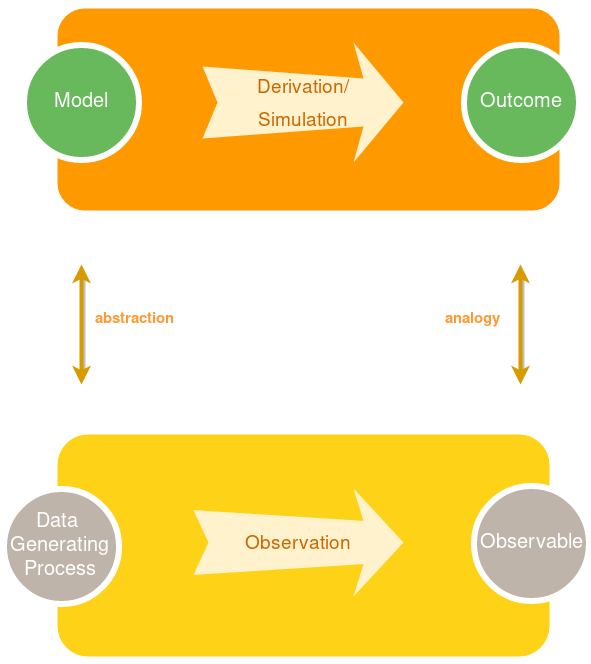
\includegraphics[scale = 0.5]{ims/ms.png}
  \caption{Relação entre Modelos e Sistemas Alvo.}
  Fonte: Adaptado de \citeonline{downey2012think}
\end{figure}

O estudo formal da ação e escolha coletiva teve como período de fundação moderno
o período entre \citeonline{black1948rationale} (marco no estudo da escolha coletiva)
e \citeonline{olson1965logic} (marco para os estudos da ação coletiva), embora
\textit{insights} típicos da literatura, como paradoxos da agregação ou o
problema do caroneiro, tenham sido discutidos anteriormente por pensadores como
Plínio, o Jovem (64-114 d.C.); Ramon Lull (1232-1315); David Hume; e John Stuart
Mill \cite{mclean2015strange, sep-free-rider, ordeshook1990emerging}. 


Embora não seja a única forma de se modelar formalmente fenômenos políticos,
modelos de escolha racional são em larga medida os mais comuns
\cite{austen1998social}. De uma forma geral, os modelos da Teoria da Escolha
Racional, em política, buscam representar fenômenos segundo alguma variante da
seguinte equação, a Equação de Plott \cite{munger2015choosing,
  ostrom1986agenda}\footnote{Essa ``equação'' é conceitual. \(\oplus\) é usado como
  um operador abstrato não especificado \cite{ostrom1986agenda}. }:
\begin{figure}[H]
\begin{align*}
  \text{Preferences} \oplus \text{Beliefs}  \oplus  \text{Physical Possibilities} \oplus \text{Institutions} = \text{Outcomes}
\end{align*}
\end{figure}
Esses modelos podem ser dividido em duas variantes: \textit{thin} ou
\textit{thick} \cite{hechter1997sociological, green1996pathologies}. Ambos os
tipos de modelos são construídos com base nos pressupostos mínimos de um modelo
de ator racional: preferências racionais e racionalidade bayesiana
\cite{gintis2016individuality}. A diferença entre eles é que os modelos
\textit{thin} não fazem pressupostos substantivos sobre os valores e objetivos
dos agentes. Neles os teóricos buscam modelar a combinação entre agentes e
instituições da maneira mais geral possível. Já modelos \textit{thick} adicionam
um conjunto de pressupostos extras sobre objetivos, valores, incerteza, com o
objetivo de representar fenômenos particulares como o comparecimento às urnas, a
competição partidária, a escolha de candidatos pelo eleitorado, independência
burocrática, o efeito fiscal de constituições, dentre outros
\cite{bendor2011behavioral}.

Todo modelo formal da escolha racional em política envolve os seguintes
elementos primitivos: o conjunto $N$ de agentes, o conjunto \(X\) de
alternativas possíveis, e para cada agente em \(N\) uma descrição de suas
preferências em relação às alternativas em \(X\) \cite[p.
263]{austen1998social}.

A preferência é uma relação de comparação de valor, onde dois conceitos são
fundamentais: o de melhor (preferência estrita), denotado por \(\succ\),  e o de igual
em valor (indiferença), denotado por \(\sim\). As seguintes propriedades definem a
noção lógica de relação de preferência \cite{sep-preferences}:

\begin{enumerate}
\item \textit{Assimetria da preferência}: \( x \succ y \to \neg (y \succ x )\); 
\item \textit{Simetria de indiferença}: \(x \sim y \to  y \sim x\); 
\item \textit{Reflexividade da indiferença }: \(x \sim x\); 
\item \textit{Incompatibilidade entre preferência e indiferença}: \(x \succ y \to \neg ( x
  \sim y)\).
\end{enumerate}

A relação de preferência fraca \( \succeq \)pode ser definida da seguinte forma:

\begin{align*}
  \text{x} \succeq y \leftrightarrow x \succ y \lor x \sim y
\end{align*}

A aplicação dessa definição de preferência no modelo do ator racional pressupõe
que ela seja uma relação binária no conjunto de alternativas \(X\), com as
seguintes propriedades, para todo \(x,y,z\) $\in$ \(X\), e para todo conjunto
\(Z\) $\subset$ \(X\) \cite{gintis2016individuality,
  binmore2008rational}:



\begin{enumerate}
\item \textit{Completude}: \(\{ x \succeq y | X \}\) ou \(\{ y \succeq x | X \}\);
\item \textit{Transitividade}: \( \{x \succeq y | X\} \) e \(\{y \succeq z | X \}\) tem por
  implicação \(\{x \succeq z | X\}\);
 \item \textit{Independência das alternativas irrelevantes}: para \(x,y,z \in Z\),
   \(\{x \succeq y | Z \}\) se e somente se \(\{x \succeq y | X\}\).
\end{enumerate}

Um pressuposto adicional é que existe um \(x \in X\) tal que para todo \(y \in X\),
\(x \succeq y\), e que num ambiente sem restrição os atores escolhem essa alternativa
\cite{gintis2009bounds}. Esses pressupostos constituem o primeiro princípio do
modelo do ator racional: os agentes possuem \textit{preferências consistentes ou
racionais}.

Uma conveniência analítica é representar relações de preferência por meio de
funções de utilidade, que são funções que atribuem um número real para cada
elemento do conjunto de alternativas \cite{sep-preferences}. A relação \( \succeq\) é
representada pela função \(u\): \(X \longrightarrow \mathbb{R}\) se e somente se:

\begin{align*}
  u(x) \geq u(y)
  \text{ se e somente se }
  x \succeq y
\end{align*}

Por meio dessa representação podemos dizer que os atores agem \textit{como se}
estivessem maximizando sua função de utilidade tendo em vista o fato da alternativa
preferida, ou ótima, para um ator $i \in N$ ser dada por \cite{binmore2008rational}:
\[\max_{\substack{x \in  X}}
  u_i(x)
\]

Importante notar que funções de utilidade são um dispositivo matemático. Modelar
agentes por meio de funções de utilidade não implica que eles sejam egoístas,
instrumentais, utilitários, hedonistas, ou que estejam ``tentando maximizar sua
utilidade'' \cite{gaus2007philosophy}.

O segundo princípio dos modelos de ator racional é a \textit{racionalidade
  bayesiana} \cite{gintis2016individuality}. Quando as alternativas são
probabilísticas primeiro pressupomos que os agentes tem um \textit{modelo do
  mundo} \cite{acemoglu2011opinion}: os agentes vão ter uma crença, representada
por meio de uma função de distribuição de probabilidade, a qual vai atribuir uma
probabilidade \(p\) para cada evento em \(X\). O modelo da escolha racional
então pressupõe que as crenças dos agentes são coerentes ou consistentes, o que
equivale a dizer que estão em conformidade com os axiomas da probabilidade
\cite{jackman2009bayesian}.

O outro elemento do princípio da racionalidade bayesiana é a \textit{atualização
  bayesiana}\cite[p.104]{gintis2016individuality}: os agentes atualizam suas
crenças segundo a Regra de Bayes.Suponha que um agente quer atualizar sua crença
sobre uma alternativa \(x \in X\), tendo em vista a observação de um dado \(m\).
Se ele atualizar sua crença segundo o pressuposto de atualização bayesiana temos
que:

\begin{align*}
  p(x|m) =
  \frac{p(m|x)
  p(x)}
  {\int p(m|x)
  p(x)
  dx}
\end{align*}

Um corolário de agentes que têm preferências e crenças consistentes, é que vão
agir segundo o \textit{princípio da utilidade esperada}
\cite{sep-rationality-normative-utility}. Para tal pressupõe-se que agentes vão
ter uma relação de preferência sobre \textit{apostas} \cite{jehle2001advanced},
onde o conjunto de apostas \(\mathcal{G}\) em \(X = \{ x_1, \ldots, x_n \}\) é dado
por:

\begin{align*}
  \mathcal{G} \equiv \big{\{}
  (p_1 \circ x_1, \ldots, p_n \circ x_n  )
  | p_i \geq 0,
  \sum_{i = 1 }^n p_i
  = 1  \big{\}}  
\end{align*}

Sendo assim, quando as alternativas são probabilísticas a utilidadde \(u:
\mathcal{G} \to \mathbb{R} \) do agente é
\cite{jehle2001advanced,sep-rationality-normative-utility}:

\begin{align*}
  u(\mathcal{G}) = \sum_{i =1}^n p_i u(x_i)
\end{align*}

Sumarizando, os modelos de escolha racional na sua versão mais básica pressupõem
agentes com preferências consistentes, o que implica que sejam transitivas,
completas e independente de alternativas irrelevantes. Caso o contexto de
decisão seja incerto também pressupõem que os agentes tem uma crença em
conformidade com os axiomas da probabilidade, suas preferências podem ser
representadas por meio de funções de utilidade esperada e atualizam suas crenças
de acordo com o Teorema de Bayes.


\section{Teoria Política Espacial}

Dentre as várias formas de modelar política por meio do modelo do ator racional
a a principal é o conjunto de modelos conhecido como Teoria Espacial (ou
Geométrica\footnote{Vamos usar o termo geométrico de maneira intercambiável com
  espacial, pelo fato do último gerar a confusão com trabalhos relacionados ao
  papel do espaço geográfico em política \cite{ward2002spatial,
    poole2005spatial}.}) de Política \cite{van2005political}.

A Teoria Espacial de Política tem suas origens nos trabalhos canônicos de Duncan
Black e Anthony Downs, e as bases matemáticas da teoria foram desenvolvidas por
Otto Davis, Melvin Hinich e Peter Ordeshook \cite{black1958theory,
  downs1957economic, poole2005spatial, miller2015spatial}. Ela está fundamentada
na idéia essencial que as alternativas, posicionamento e preferências dos
agentes políticos podem ser representadas por meio de espaços geométricos. Ela
captura a metáfora e noção da linguagem política diária de que as alternativas
políticas tem uma relação de proximidade/distância, tal qual a noção de que
partidos, pessoas, ou propostas são de ``extrema-esquerda'', ``centristas'' ou
``de direita'' \cite{munger2015choosing}.


Seguindo \citeonline{humphreys2010spatial}, podemos dividir os modelos
geométricos em dois grupos. Eles podem ser \textit{fracamente} ou
\textit{fortemente} espaciais. Os modelos fracamente espaciais só caracterizam
as alternativas e as preferências segundo uma analogia geométrica. Já modelos
fortemente espaciais envolvem uma teoria comportamental sobre como as pessoas
pensam sobre política \cite{laver2014measuring}.


Nos modelos fracamente espaciais o conjunto de alternativas \(X\) é pensado como
um espaço, mais comumente como o subconjunto de um espaço Euclidiano de \(n\)
dimensões \cite{austen1998social}. Assumem também que agentes tem preferências,
consistentes, sobre esse espaço. Seguindo o primeiro princípio do ator racional,
isso significa que a alternativa preferida para cada agente \(i \in N\) pode ser
pensada como um ponto no espaço. Essa alternativa $x_i$ é o \textit{ponto ideal}
do agente. Não assume-se, contudo, que os agentes percebem as utilidades das
alternativas em termos das distâncias relativas no espaço subjacente. Os agentes
têm funções de utilidade abstratas, não especificadas
\cite[p.14]{humphreys2010spatial}.

Modelos fortemente espaciais, por outro lado, pressupõe que os agentes tem uma
cognição geométrica. Isso significa que localizam as alternativas no espaço, e
ranqueiam as alternativas segundo uma medida de distância \(d_i\). A função de
utilidade dos agentes é a composição da função de distância e uma função de
perda de forma que \(u_i(y) = f_i(d_i(x_i,y)) \).

O pressuposto modal  é que métrica é Euclidiana: os agentes
medem a distância entre dois pontos no espaço de alternativas usando o Teorema
de Pitágoras \cite{munger2015choosing}. Ademais, assume-se funções com um único
pico ( o ponto ideal do agente) e simétricas. Funções de utilidade comumente
usadas na ciência política são a linear, a quadrática e a gaussiana, ilustradas
na  Figura 2: 


\begin{figure}[H]
  \centering 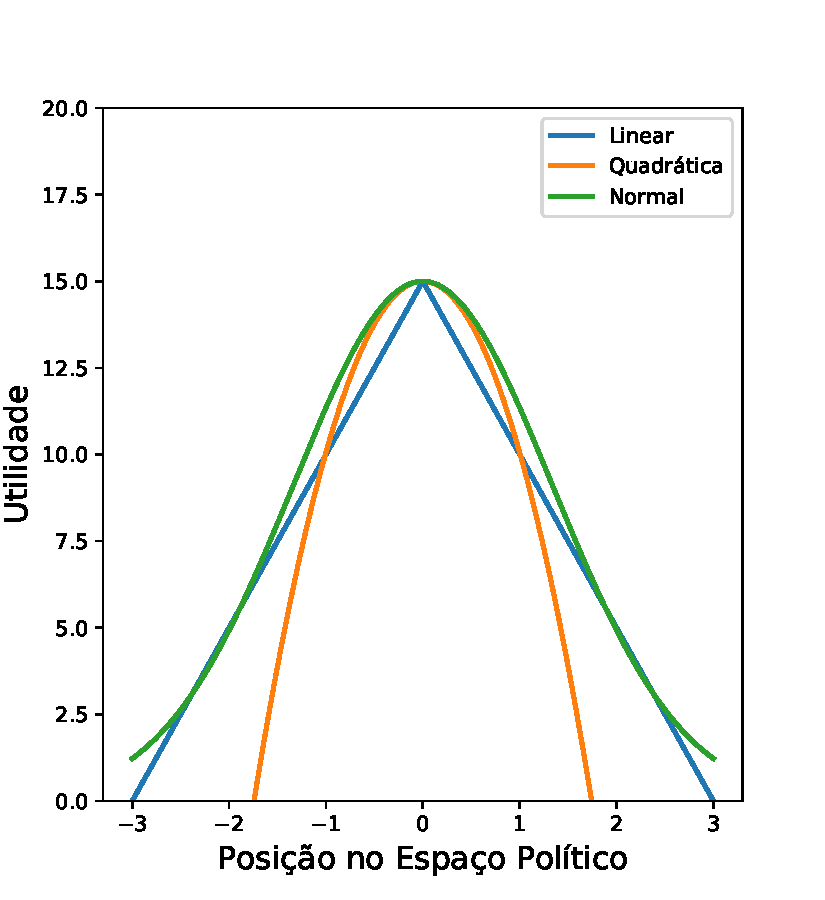
\includegraphics[scale = 0.6]{ims/utilities.pdf}
  \caption{Funções de Utilidade comuns em Política}
  Fonte: Adaptado de \citeonline{armstrong2014analyzing}
\end{figure}

Essa estrutura básica do modelo espacial é aplicada em dois tipos de fenômenos:
votos em comitê e eleições de massa \cite{munger2015choosing}. Há, contudo, uma
grande diferença entre essas duas situações de ação, e essa diferença motiva
nosso problema.


\section{Teoria Espacial e Eleições}


A diferença entre os dois contextos de ação é reconhecida desde as contribuições
seminais de Black e Downs. Em votos em comitê o número de agentes é pequeno, os
agentes são bem informados e  a decisão costuma ter alta implicação para eles.
Já em eleições de massa existem muitos eleitores, a informação sobre as
alternativas é ambígua e os efeitos da decisão são difusos.

Essa distinção tem por corolário uma maior conformidade do voto em comitês com
os \textit{pressupostos de similaridade} entre um modelo de ator racional e uma
situação de interesse alvo. A modelagem de sistemas sociais exige uma atenção
quanto a plausibilidade da analogia entre modelo e sistema alvo
\cite{de2005computational}, tanto no tocante ao contexto de escolha dos agentes
quanto ao seu comportamento \cite{page2008uncertainty}. Disso segue que o modelo
do ator racional, mesmo na sua versão mais \textit{thin}, não é universalmente
aplicável. Isto é, não espera-se que em toda situação social os atores ajam de
forma racional.


O primeiro pressuposto de similaridade refere-se a propriedades dos agentes alvo:
as crenças e preferências deles são independentes \cite{binmore2008rational}. Os
outros três lidam com o contexto de ação alvo: a situação de ação é simples,
tanto em estrutura, quanto informacionalmente; os agentes têm incentivo para
agir e informar-se; e há tempo disponível para os agentes aprenderem
\cite{binmore2007work, page2008uncertainty}.

A aplicação do modelo racional ao contexto do comportamento eleitoral é assim
não trivial, por uma razão: a escala. Como argumenta \citeonline{binmore2008rational}
a aplicação do modelo da decisão racional em  ``large worlds'' é problemática,
pois provavelmente estaremos violando algum dos pressupostos de similaridade
apresentados.

Desde seu surgimento o programa de pesquisa ``Downsiano'' reconhece a distância
entre a aplicação ideal, do ponto de vista preditivo, e o sistema alvo,
eleições. \citeonline{downs1999teoria} dedica uma grande porção do livro à
incerteza e a problemas de incentivos, e a obra inspirou uma ampla literatura
sobre comparecimento às eleições, tomada de decisão do eleitor e competição
partidária \cite{bendor2011behavioral}.

Em relação à tomada de decisão do eleitor há uma tensão entre a literatura em
teoria formal e a literatura em psicologia política: a primeira costuma
pressupor que agentes têm ideologias bem definidas e são bem informados, ou tem
alguma noção probabilística, sobre as alternativas partidárias, algo contestado
veementemente pela segunda \cite[p.5]{bendor2011behavioral}. A falta de
conhecimento sobre temas/questões e a instabilidade de resposta a
\textit{surveys} é um dos resultados recorrentes na literatura em opinião
pública desde sua fundação \cite{berelson1952democratic, converse2006nature,
  zaller1992simple, kuklinski2000misinformation}.

A instabilidade nas resposta e a suscetibilidade dos cidadãos a \textit{framing
  effects}\footnote{\textit{Framing effects} são ``situações nas quais formas
  alternativas de apresentar uma questão política levam a diferentes respostas
  do público'' \cite[p.56]{bartels2003democracy}.} levam
\citeonline{bartels2003democracy} a contestar o uso da noção de preferência como
base para o estudo do nexo democrático, pois cidadãos não teriam preferências
consistentes, coerentes ou estáveis. Ele argumenta, contudo, que os eleitores
têm posicionamentos, os quais são melhor teorizados como
\textit{atitudes}\footnote{ Ele define atitude como uma tendência psicológica
  que é expressa pela avaliação de uma entidade particular com algum grau de
  aprovação ou desaprovação \cite[p.52]{bartels2003democracy}.}.

Embora possa-se contestar a validade externa dos questionários que buscam
demonstrar a instabilidade de posicionamento dos cidadãos
\cite{druckman2012public}, e a relevância dos \textit{framing effects} para a
aplicação modelo do ator racional \cite[p. 107]{gintis2016individuality},
Bartels levanta um ponto incontornável: o pressuposto de preferências racionais
não é inócuo, em especial no contexto eleitoral.

O pressuposto de que agentes têm preferências racionais sobre todas questões
políticas é exigente do ponto de vista cognitivo. Contudo, não é necessário.
Para aplicar o modelo geométrico de política em um contexto macro não é
necessário supor que cada questão (\textit{issue}) vá definir uma dimensão no
espaço de alternativas. O que é necessário é que os agentes tenham
\textit{algum} posicionamento nas questões, e que exista uma interrelação entre
a resposta do eleitor entre posicionamentos, de forma que possamos descrever as
atitudes dos agentes em todas as questões segundo a correlação com alguma
dimensão latente \cite{poole2005spatial,laver2014measuring}.
\citeonline{poole1985ideology} encontra que $80\%$ dos votos no Congresso
americano podem ser explicados por uma única dimensão latente
(liberal-conservador). Já \citeonline{benoit2006party} encontra que no máximo
três dimensões são necessárias para capturar a informação relevante sobre os
posicionamentos dos eleitores, em um banco de dados de 47 países.

A preferência dos agentes nessas dimensões é, portanto, construída a partir do
posicionamento, atitudes, considerações, opiniões e crenças, deles num
agrupamento de questões. Isso significa que as preferências dos eleitores são
\textit{extrínsecas}. Preferências intrínsecas são preferências irredutíveis.
Independem de mudanças do ambiente ou de alguma razão em particular. O agente
\(i\) simplesmente prefere \(x\) a \(y\). Já preferências extrínsecas dependem
de um julgamento, uma crença, de que uma alternativa, é, em algum sentido, melhor
que a outra. Preferências extrínsecas têm razões subjacentes, e, portanto,
possivelmente mudam quando ocorrem mudanças no ambiente \cite{liu2010wright,
  binmore2008rational}.

Preferências extrínsecas violam o pressuposto de que as preferências e crenças
dos agentes são independentes, o que complica a análise da situação de ação por
meio do modelo do ator racional, dado que não podemos pressupor que elas são
estáveis. Como as preferências no contexto eleitoral necessariamente são
construídas a partir de posicionamentos num conjunto de questões, por definição,
elas são extrínsecas. Logo, são, potencialmente, sensíveis à mudanças no
ambiente.Tendo em vista tanto a complexidade informacional do contexto, quanto
os baixos incentivos à busca de informação, isso vai significar que os agentes
serão \textit{incertos} quanto às suas preferências. Essa incerteza em relação
às preferências, e o baixo custo, percebido, da mudança permitem que modelos de
dinâmicas de opinião\footnote{Área a ser discutida no Capítulo 2.} possam ser
usados para representar seu processo de formação e cristalização.


As preferências dos cidadãos, portanto, não vão ser estáticas.Isso não
significa, contudo, que elas necessariamente serão altamente instáveis. Como
as preferências são construídas a partir de um conjunto de posicionamentos e
crenças em várias questões, é de se esperar que elas sejam mais estáveis do que
o posicionamento dos atores em cada questão específica, o objeto dos estudos em
opinião pública que têm por objetivo analisar a instabilidade de resposta dos
eleitores \cite{druckman2012public}. Do ponto de vista macro, é de se esperar,
desta forma, que a distribuição de preferência dos eleitores seja consistente. A
Figura 3, a qual mostra o auto-posicionamento político, numa escala de 0 a 10
(esquerda-direita), de respondentes\footnote{A cada edição uma nova amostrada é
  selecionada.} em sete edições do \textit{European Social Survey},
condiz\footnote{Para questões metodológicas em relação a esses dados ver o
  Apêndice 1.} com essa expectativa:


\begin{figure}[H]
  \centering 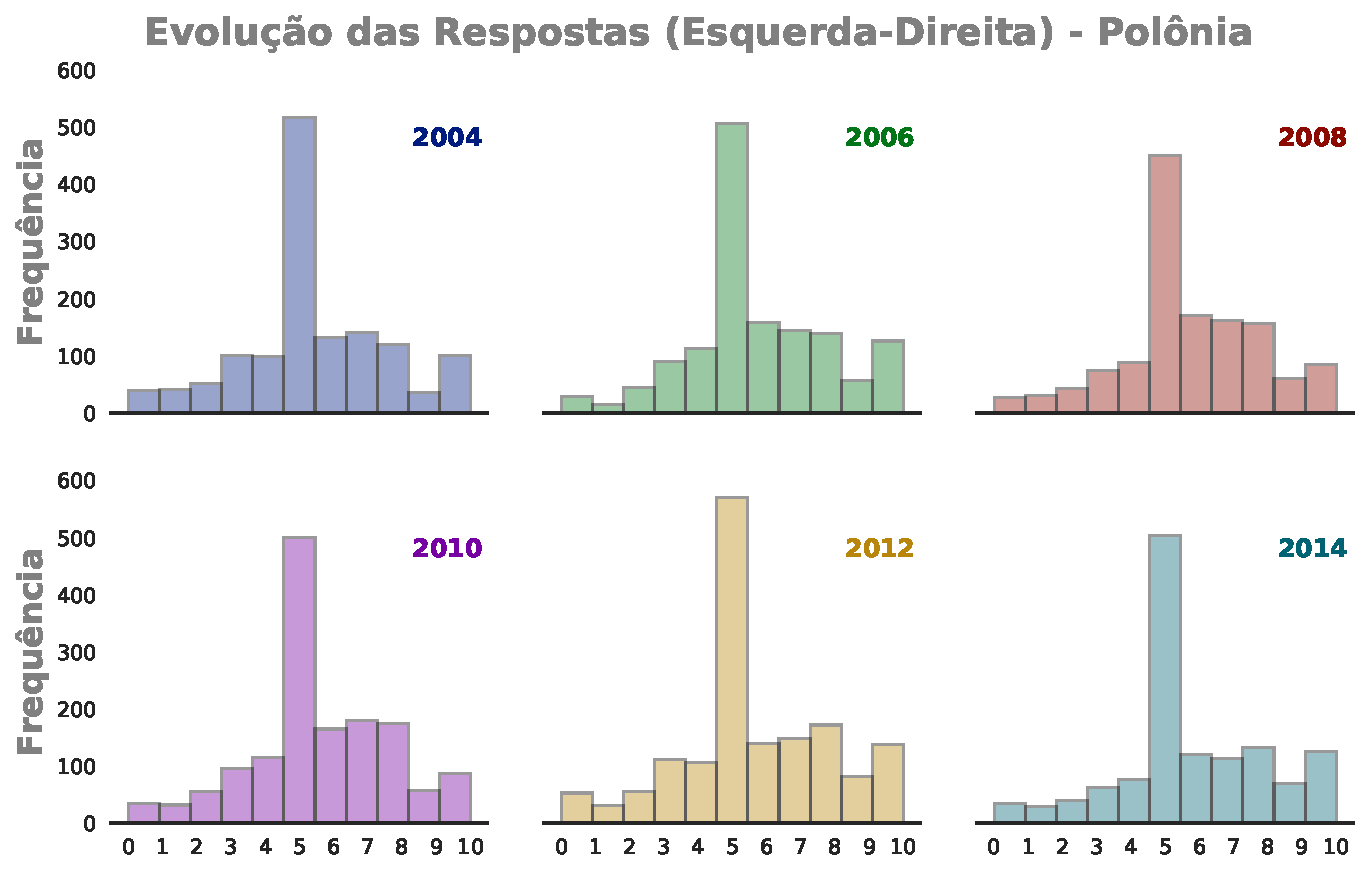
\includegraphics[scale = 0.8]{ims/ess_Pol_plots.pdf}
  \caption{Evidência de estabilidade ideológica}
  Fonte: Dados do \textit{European Social Survey}
\end{figure}



A escala do fenômeno eleitoral também afeta uma segunda categoria de agentes: os
partidos. Os partidos também estão posicionados no espaço de alternativas \(X\)e
competem pelos votos dos eleitores. Para os partidos \(X\) é um espaço de
plataformas. Para competirem têm de ser capazes de determinar qual o percentual
de votos das posições nesse espaço. A literatura reconhece que talvez os
partidos não sejam capazes de fazê-lo, adicionando a possibilidade de que eles
sejam incertos quanto as preferências políticas dos eleitores
\cite{glazer1989model, grofman2004downs}.


Como argumenta \citeonline[p.144]{page2008uncertainty} essa é a estratégia
\textit{one-theta-fits-all} , que consiste em ignorar a dificuldade da tomada de
decisão e a complexidade do ambiente em que os agentes estão situados, e
modelá-los como otimizadores sob incerteza. Para a competição espacial com
dimensão $n>1$, demonstra \citeonline[14-27]{laver2011party}, agir de maneira
ótima, é, contudo, impossível. Os partidos, desta forma, necessariamente agem
segundo heurísticas e se movimentam no \textit{electoral landspace} de forma
adaptativa \cite{kollman1998political, de1999adaptive}. Isso abre a
possibilidade, teórica, de que os partidos fiquem presos em picos locais. Do
ponto de vista empírico, a Figura 4 dá suporte à essa possibilidade:

\begin{figure}[H]
  \centering 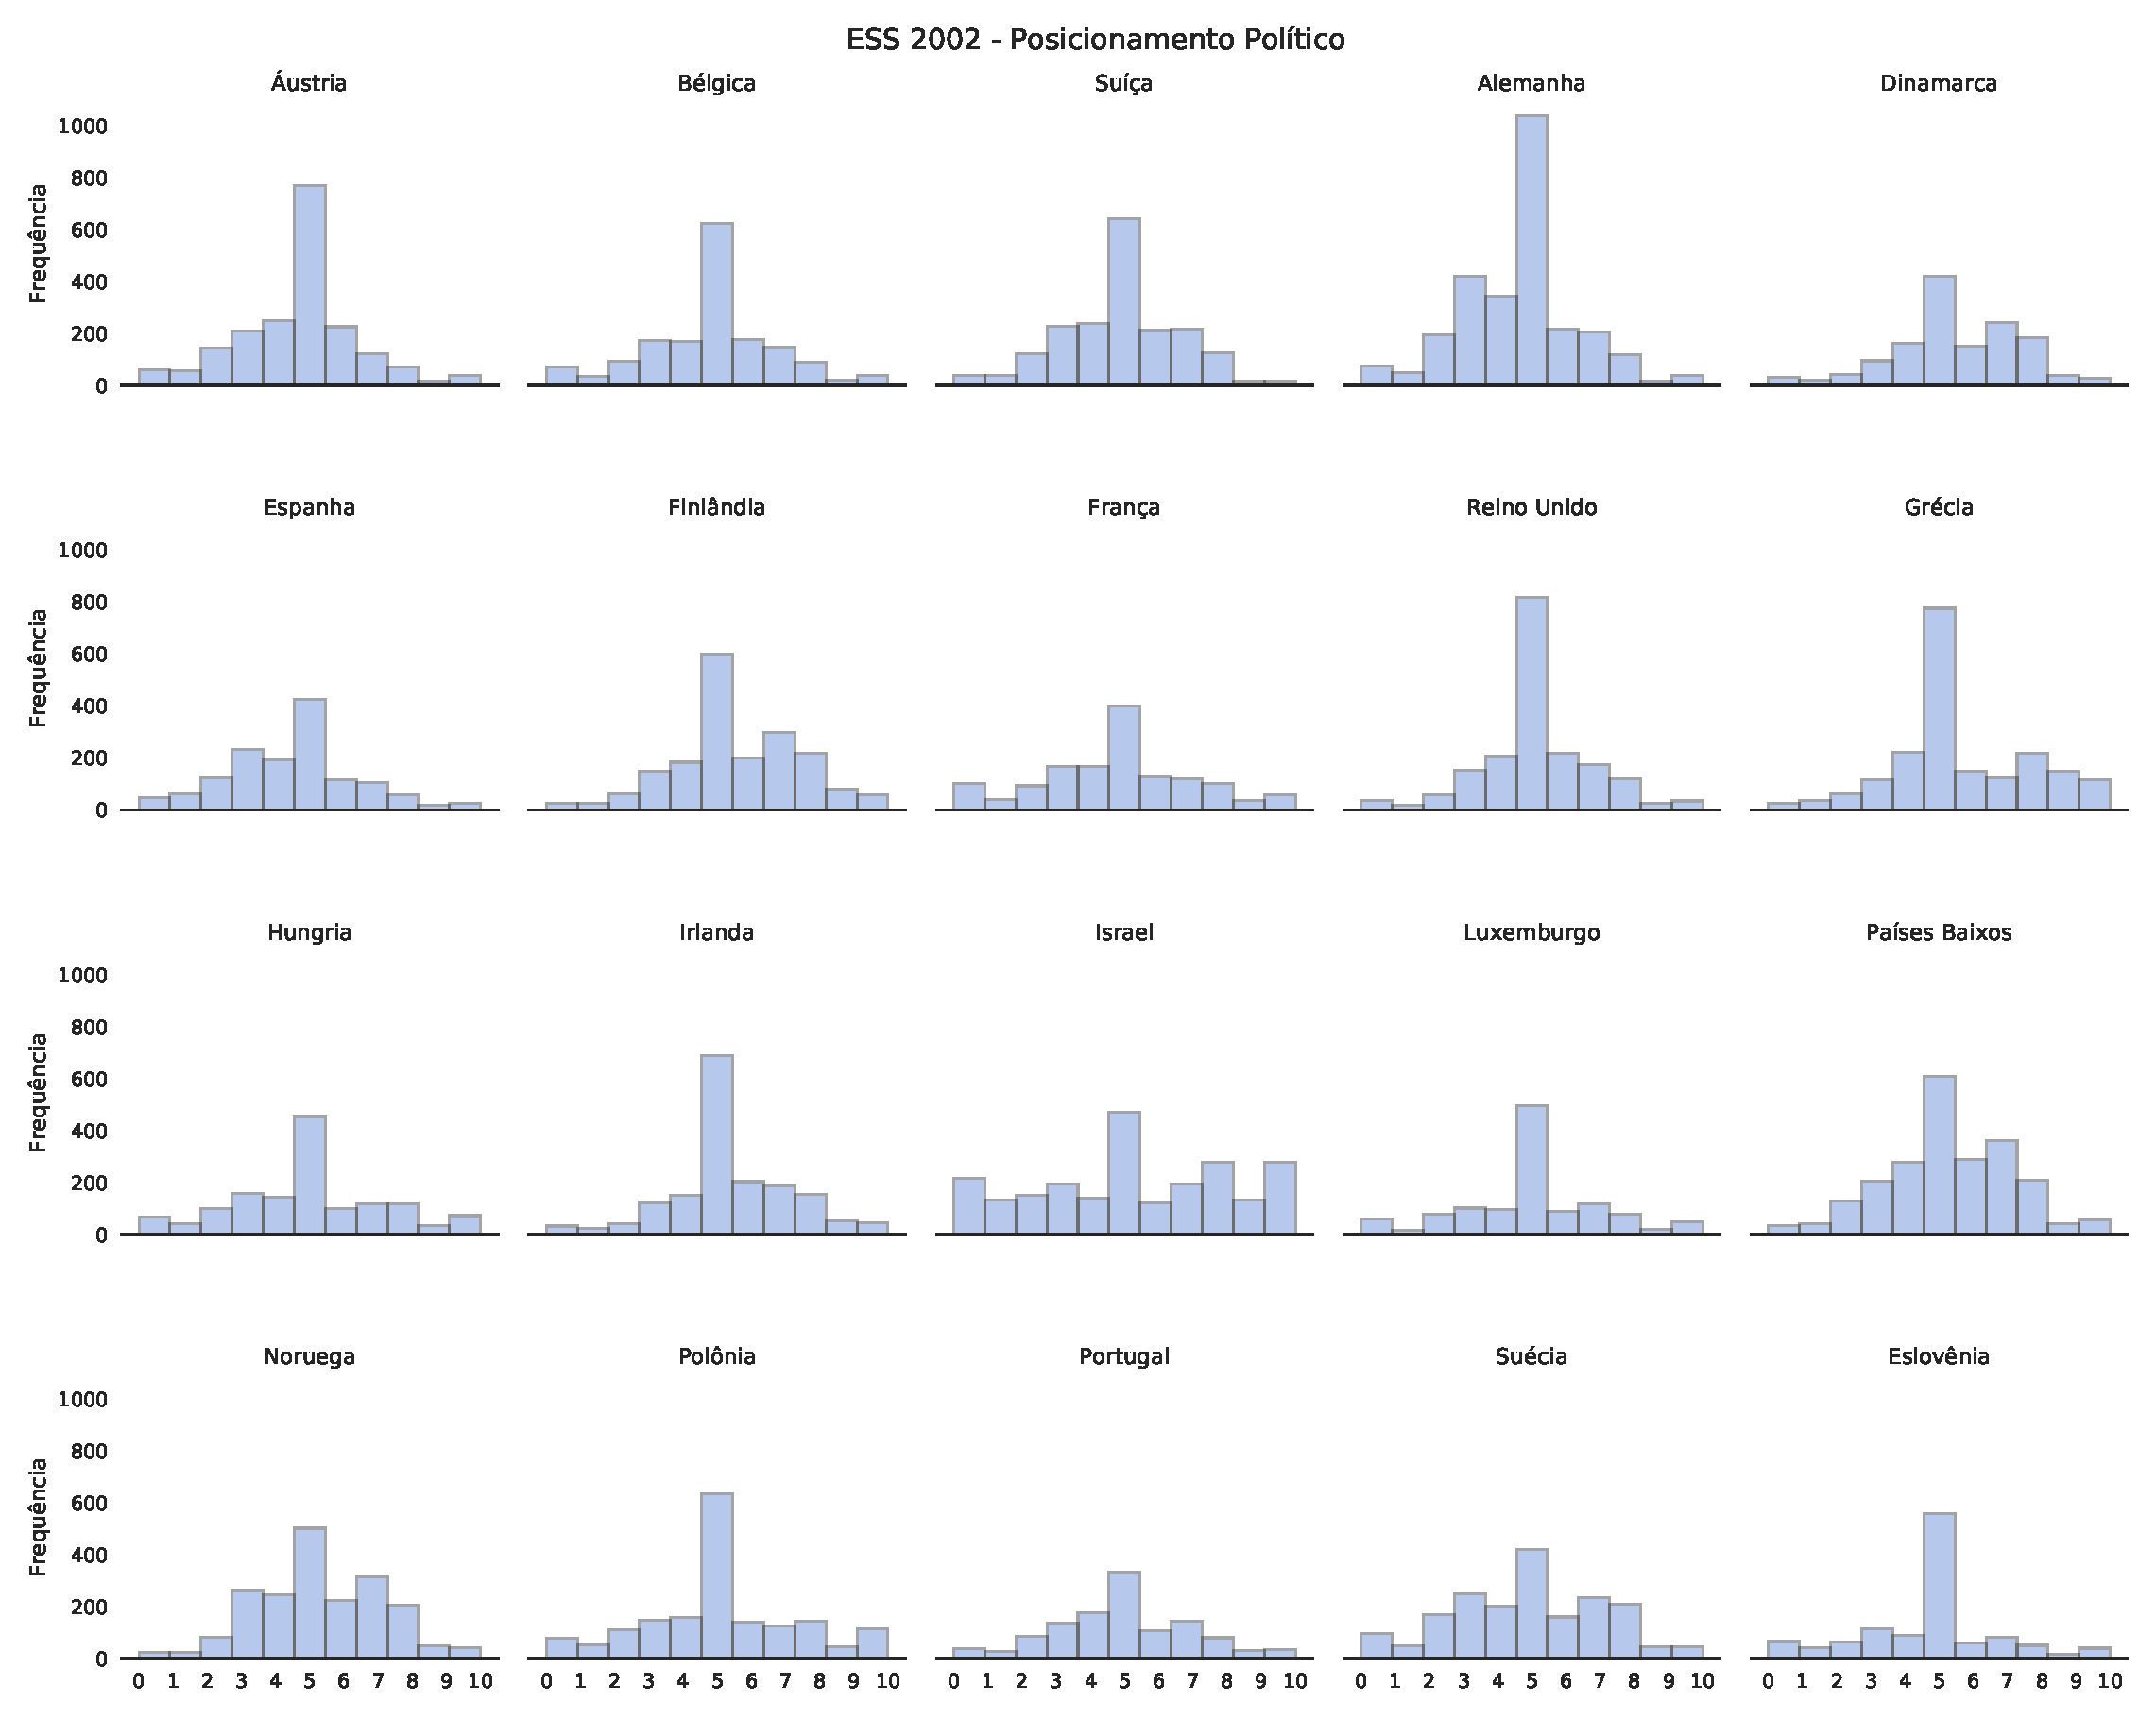
\includegraphics[width=\textwidth,
  height=12cm]{ims/ess_2002_plots.pdf}
  \caption{Evidência de distribuição ideológica  com múltiplos picos}
  Fonte: Dados do \textit{European Social Survey} (primeira edição)
\end{figure}

Dado que as eleições são o principal mecanismo de conexão entre cidadãos e
governo nas poliarquias \cite{dahl1989democracy} e dado que a sobrevivência dos
partidos na competição eleitoral depende da sua capacidade de captar o voto dos
eleitores, podemos concluir que o \textit{formato} da distribuição das
preferências dos eleitores é central para o estudo do nexo democrático.

Temos, desta forma, duas diretrizes para o estudo. Do ponto de vista micro,
podemos modelar os pontos ideais dos agentes segundo um modelo de dinâmicas de
opinião. Esse é o nosso ponto de partida. Do ponto de vista macro, aspiramos que
nossos modelos consigam gerar distribuições que sejam plausíveis do ponto de
vista empírico, dado que o formato delas importa. Esse é o nosso \textit{benchmark}.




